\documentclass{article}

\usepackage{Sweave}
\begin{document}
\Sconcordance{concordance:Lab2.tex:Lab2.Rnw:%
1 2 1 1 0 15 1 1 2 1 0 2 1 11 0 1 1 3 0 1 2 2 1 1 2 1 0 1 1 4 0 1 2 4 1 %
1 2 1 0 1 1 5 0 1 1 5 0 1 1 6 0 1 2 8 1 1 2 1 0 1 1 22 0 1 2 2 1 1 2 9 %
0 1 2 10 1 1 2 1 0 1 1 23 0 1 2 2 1 1 2 1 0 3 1 4 0 1 2 3 1 1 2 1 0 3 1 %
3 0 1 2 2 1 1 2 1 0 1 1 3 0 1 2 2 1 1 2 1 0 4 1 5 0 1 1 6 0 1 2 9 1 1 2 %
13 0 1 2 18 1 1 7 9 0 1 2 2 1 1 3 2 0 2 1 27 0 1 2 22 1}



\textbf{Linear Regression in R}\\[.25cm]

Here will illustrate how linear regression works in R.  We will want to make sure everyone is comfortable with  multiple linear regression in general.  Remember, we use the following notation to show the relationship between \\[.25cm]

\begin{eqnarray*}
\mu_y&=\beta_0 + \beta_1 x_1 + \beta_2 x_2 + \ldots\\
\end{eqnarray*}

Here we are using our $x_1$, $x_2$, etc. (explanatory variables) to predict a particular response variable $y$, where $\mu_y$ is the average response for a set of observed values for the explanatory variables.\\[.25cm]

We will use the diamonds dataset built into the \textbf{ggplot2} package to illustrate multiple linear regression in R.  We installed the ggplot2 library during the first class.  You can see the top of the dataset we will be using by typing the following commands.\\

\begin{Schunk}
\begin{Sinput}
> library(ggplot2)
> attach(diamonds)
> head(diamonds)
\end{Sinput}
\begin{Soutput}
  carat       cut color clarity depth table price    x    y    z
1  0.23     Ideal     E     SI2  61.5    55   326 3.95 3.98 2.43
2  0.21   Premium     E     SI1  59.8    61   326 3.89 3.84 2.31
3  0.23      Good     E     VS1  56.9    65   327 4.05 4.07 2.31
4  0.29   Premium     I     VS2  62.4    58   334 4.20 4.23 2.63
5  0.31      Good     J     SI2  63.3    58   335 4.34 4.35 2.75
6  0.24 Very Good     J    VVS2  62.8    57   336 3.94 3.96 2.48
\end{Soutput}
\begin{Sinput}
> ?diamonds
\end{Sinput}
\end{Schunk}

Here, we can use the \textbf{pairs()} to look at the relationship between all variables.  The last three variables in this dataset are not of interest and I am not interested in using the $table$ column either.  Therefore, I am going to remove these columns, which can be done as shown below.\\[.25cm]

\begin{Schunk}
\begin{Sinput}
> diamonds = diamonds[c(-6, -8, -9, -10)]
> pairs(diamonds[c(1,5,6)])
\end{Sinput}
\end{Schunk}
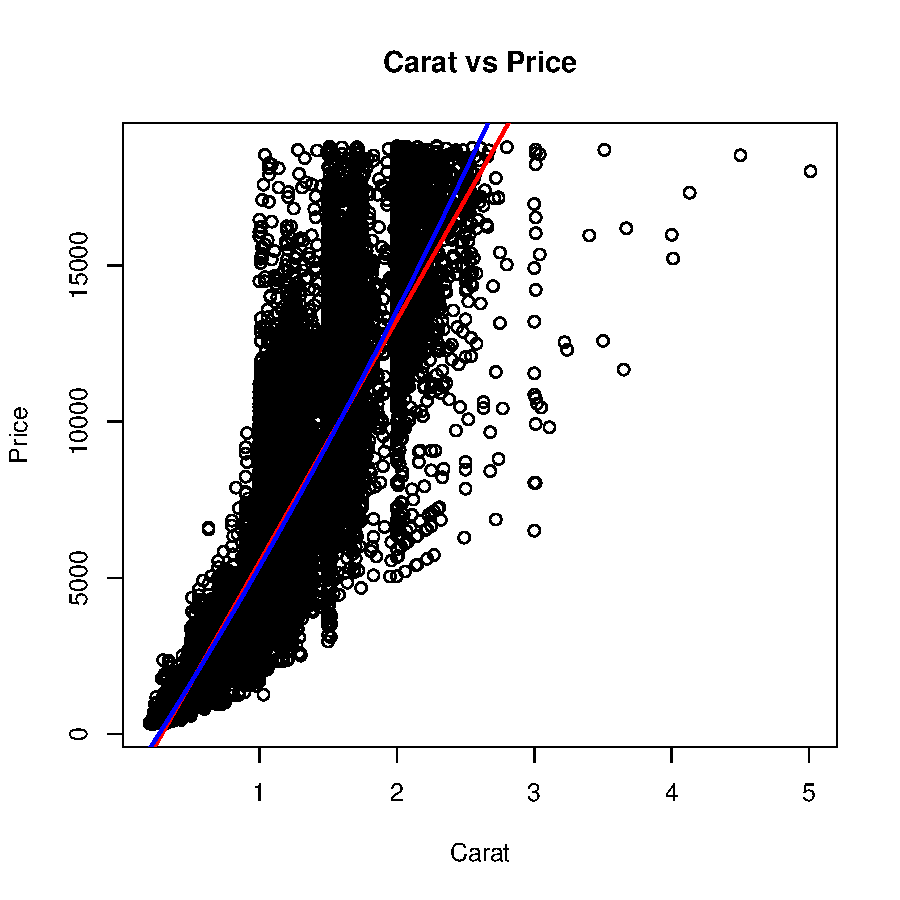
\includegraphics{Lab2-chunk}

Running the \textbf{dim()} command shows that we have more than 53 thousand rows.  Because there are so many rows, the \textbf{pairs()} command may take a little time to run.  I ran this command only between the 'non-categorical' variables. We can see that there is a relationship between carat and price.  However, we don't (visually) seem to have a relationship between the other variables (table and price, nor carat and table).  

We can estimate the model, using the \textbf{lm()} function.  We should do more EDA in a real world situation: look at the summary of each variable, histograms, bar charts, etc. For the purpose of not making this too long, I won't spend time looking at all the EDA I would generally look at before fitting any sort of model.  To address the direction of this lab (linear regression), we could look at correlations between the quantitative variables.

\begin{Schunk}
\begin{Sinput}
> attach(diamonds)
> cor(carat, table)
\end{Sinput}
\begin{Soutput}
[1] 0.1816175
\end{Soutput}
\begin{Sinput}
> cor(carat, price)
\end{Sinput}
\begin{Soutput}
[1] 0.9215913
\end{Soutput}
\begin{Sinput}
> cor(price, table)
\end{Sinput}
\begin{Soutput}
[1] 0.1271339
\end{Soutput}
\end{Schunk}

The correlation coefficients quantify what we saw in the plot.  With the relationship between price and carat, we could start with a simple linear regression model. The theoretical model can be considered as:  

\begin{eqnarray*}
\mu_y&=\beta_0 + \beta_1 x_1 \\
\end{eqnarray*}

If we are interested in predicting price based on the carat size, we fit the following model:

\begin{Schunk}
\begin{Sinput}
> linear_model = lm(price~carat)
> summary(linear_model)
\end{Sinput}
\begin{Soutput}
Call:
lm(formula = price ~ carat)

Residuals:
     Min       1Q   Median       3Q      Max 
-18585.3   -804.8    -18.9    537.4  12731.7 

Coefficients:
            Estimate Std. Error t value Pr(>|t|)    
(Intercept) -2256.36      13.06  -172.8   <2e-16 ***
carat        7756.43      14.07   551.4   <2e-16 ***
---
Signif. codes:  0 ‘***’ 0.001 ‘**’ 0.01 ‘*’ 0.05 ‘.’ 0.1 ‘ ’ 1

Residual standard error: 1549 on 53938 degrees of freedom
Multiple R-squared:  0.8493,	Adjusted R-squared:  0.8493 
F-statistic: 3.041e+05 on 1 and 53938 DF,  p-value: < 2.2e-16
\end{Soutput}
\end{Schunk}

Based on the estimates, you should be able to interpret the intercept and slope for this model.  You can see the multiple R-squared value and adjusted R-squared value at the bottom of the summary.  We can also look at individual t-tests of each coefficient to determine the significance of a particular variable.

\begin{Schunk}
\begin{Sinput}
> anova(linear_model)[,c(-5)]
\end{Sinput}
\begin{Soutput}
             Df     Sum Sq    Mean Sq F value
carat         1 7.2913e+11 7.2913e+11  304051
Residuals 53938 1.2935e+11 2.3980e+06        
\end{Soutput}
\end{Schunk}

We can also look at the anova table to see if our overall model is useful.  We can also get the MSE from the anova table.  The information from the anova table matches the summary from the linear model.\\[.25cm]

We might want to see if a quadratic model would fit better to the data. The theoretical model will be of the following form: 

\begin{eqnarray*}
\mu_y&=\beta_0 + \beta_1 x_1 + \beta_2 x_1^2 \\
\end{eqnarray*}

We can then fit our model using the following code.  

\begin{Schunk}
\begin{Sinput}
> quad_model = lm(price~carat+ I(carat^2))
> summary(quad_model)
\end{Sinput}
\begin{Soutput}
Call:
lm(formula = price ~ carat + I(carat^2))

Residuals:
     Min       1Q   Median       3Q      Max 
-26350.0   -724.2    -35.9    445.8  12881.1 

Coefficients:
            Estimate Std. Error t value Pr(>|t|)    
(Intercept) -1832.58      21.69   -84.5   <2e-16 ***
carat        6677.03      46.40   143.9   <2e-16 ***
I(carat^2)    507.91      20.82    24.4   <2e-16 ***
---
Signif. codes:  0 ‘***’ 0.001 ‘**’ 0.01 ‘*’ 0.05 ‘.’ 0.1 ‘ ’ 1

Residual standard error: 1540 on 53937 degrees of freedom
Multiple R-squared:  0.851,	Adjusted R-squared:  0.851 
F-statistic: 1.54e+05 on 2 and 53937 DF,  p-value: < 2.2e-16
\end{Soutput}
\end{Schunk}

We could look at the way the linear model fits the data as compared to the quadratic model.

\begin{Schunk}
\begin{Sinput}
> plot(carat, price, xlab="Carat", ylab="Price", main="Carat vs Price")
> abline(linear_model, col="red", lwd=2)
> qmod <- function(x) -1832.58 + 6677.03*x +507.91 * x^2 
> curve(qmod, 0,4, add=TRUE, col="blue", lwd=2) 
\end{Sinput}
\end{Schunk}
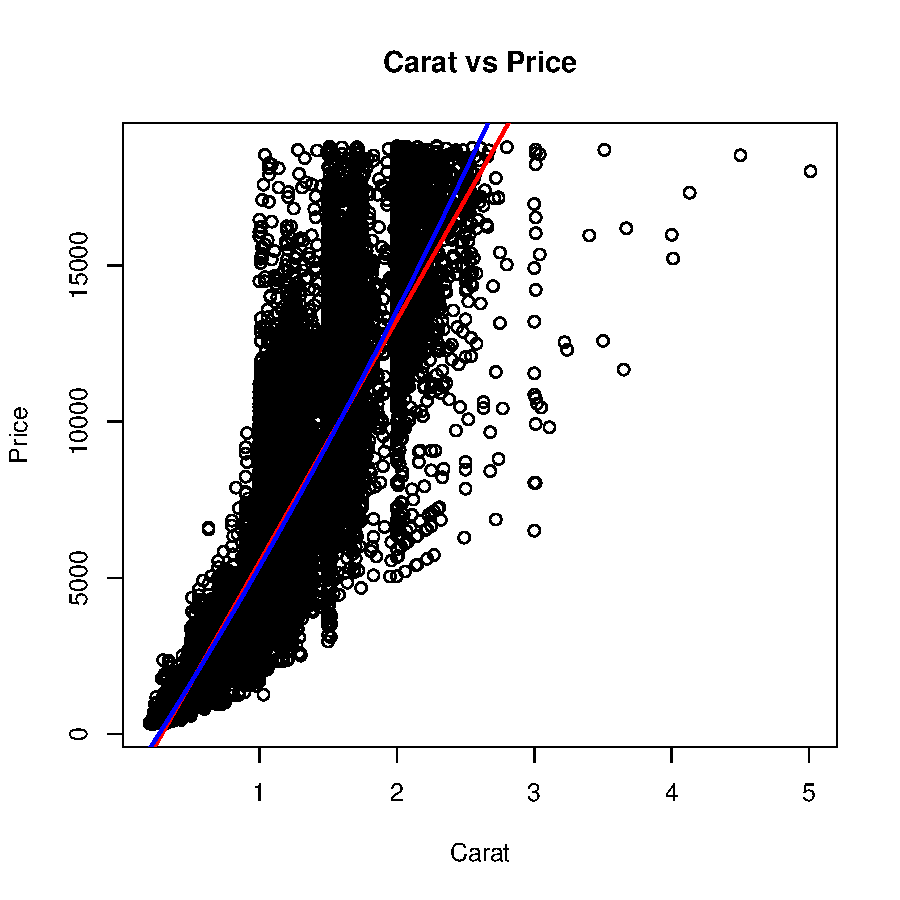
\includegraphics{Lab2-chunk}


We can see that the adjusted R-squared for the quadratic model is higher.  Both models have relatively strong R-squared values.  We might see how well the model fits when using a training-test set to test model fit.  First we would create our training and test datasets.

\begin{Schunk}
\begin{Sinput}
> set.seed(123)
> train_ind = sample(nrow(diamonds), size = nrow(diamonds)/2)
> train = diamonds[train_ind, ]
> test = diamonds[-train_ind, ]
\end{Sinput}
\end{Schunk}

We then fit both models on the training data, we can then use each model to make predictions on the test data.  We could measure the MSE from each model on the test data and compare them to choose the 'best' model.

\begin{Schunk}
\begin{Sinput}
> lin_train_mod = lm(price~carat, data=train)
> quad_train_mod = lm(price~carat + I(carat^2), data =train)
\end{Sinput}
\end{Schunk}

Here we save the predicted values from both of these models:

\begin{Schunk}
\begin{Sinput}
> lin_preds = predict(lin_train_mod, data = test)
> quad_preds = predict(quad_train_mod, data = test)
> lin_mse = mean((test$price - lin_preds)^2)
> quad_mse = mean((test$price - quad_preds)^2)
> lin_mse
\end{Sinput}
\begin{Soutput}
[1] 29241990
\end{Soutput}
\begin{Sinput}
> quad_mse
\end{Sinput}
\begin{Soutput}
[1] 29267666
\end{Soutput}
\end{Schunk}


Although, the R-squared adjusted seemed to suggest that a quadratic model was a better fit, the MSE is lower for a linear model in the above split of training vs. test data.  Using a cross-validation technique would iterate the process we just conducted with multiple splits of training and test sets to assure that our split wasn't a fluke.  We will look into these techniques more closely in future labs.  There are multiple built in methods to perform cross-validation, so that we do not have to write a loop to do it ourselves.\\[.25cm]

The text talks a little about the assumptions of modeling data with linear models.  Note that these are assumptions that are necessary for drawing inferential statements - that is saying something about the population from which the diamonds in our dataset were collected.  If we are only interested in predicting well, meeting these assumptions is not necessary.  In some cases, meeting the assumptions (such as our linear model assumption) can assist in making strong predictions.\\[.25cm]

Linear models tend not to be the best in terms of their ability to predict compared to many other types of models.  However, they are very common in many environments due to the ease of being able to interpret the results.  With this in mind, let's fit a multiple linear regression model to our data, judge the model fit, and interpret the coefficients.\\

We can look at the structure of our data (which we really should do at the beginning of the analysis), and see what variables we have to work with in building a multiple linear regression model to predict price.

\begin{Schunk}
\begin{Sinput}
> str(diamonds)
\end{Sinput}
\begin{Soutput}
'data.frame':	53940 obs. of  6 variables:
 $ carat  : num  0.23 0.21 0.23 0.29 0.31 0.24 0.24 0.26 0.22 0.23 ...
 $ cut    : Ord.factor w/ 5 levels "Fair"<"Good"<..: 5 4 2 4 2 3 3 3 1 3 ...
 $ color  : Ord.factor w/ 7 levels "D"<"E"<"F"<"G"<..: 2 2 2 6 7 7 6 5 2 5 ...
 $ clarity: Ord.factor w/ 8 levels "I1"<"SI2"<"SI1"<..: 2 3 5 4 2 6 7 3 4 5 ...
 $ depth  : num  61.5 59.8 56.9 62.4 63.3 62.8 62.3 61.9 65.1 59.4 ...
 $ price  : int  326 326 327 334 335 336 336 337 337 338 ...
\end{Soutput}
\end{Schunk}

Note, the coding used for categorical variables in R is not the same as that used in JMP.  However, the number of explanatory variables added into the model for any categorical variable is still the number of levels of the categorical variable minus one.  Therefore, if we wanted to add the cut as a predictor, we would add 4 additional explanatory variables to our model.

The theoretical model we would fit to include a linear term of carat and cut as a predictor of price will be of the following form:

\begin{eqnarray*}
\mu_y&=\beta_0 + \beta_1 x_1 + \beta_2 x_2 + \beta_3 x_3 + \beta_4 x_4 + \beta_5 x_5\\
\end{eqnarray*}

where 

\begin{itemize}
\item[] $\mu_y$ is the average price for a given set of x-values
\item[] $x_1$ is the carat value
\item[] $x_2$, $x_3$, $x_4$, and $x_5$ code the cut. 
\end{itemize}

I have defined my dummy variables in the following way for $x_2$, $x_3$, $x_4$, and $x_5$.  When I tried to fit the model directly, R was trying to add higher order terms to account for the categorical variable. For ease of interpretation, I created my own dummy variables. Note, the following code will take a little time to run.

\begin{Schunk}
\begin{Sinput}
> for (i in 1:length(cut)){
+ diamonds$x_2[i] = if(cut[i] == 'Fair'){1} else {0}
+ diamonds$x_3[i] = if(cut[i] == "Good"){1} else {0}
+ diamonds$x_4[i] = if(cut[i] == 'Very Good'){1} else {0}
+ diamonds$x_5[i] = if(cut[i] == "Premium"){1} else {0}
+ }
\end{Sinput}
\end{Schunk}

Before fitting our model, I will make the column names for our 'x' variables more intuitive.  Then fitting our model we have:

\begin{Schunk}
\begin{Sinput}
> names(diamonds) = c("carat","cut","color","clarity","depth",
+                     "price","Fair","Good","VeryGood","Premium") 
> mlr_mod = lm(price~carat+Fair+Good+VeryGood+Premium, data=diamonds)
> summary(mlr_mod)
\end{Sinput}
\begin{Soutput}
Call:
lm(formula = price ~ carat + Fair + Good + VeryGood + Premium, 
    data = diamonds)

Residuals:
     Min       1Q   Median       3Q      Max 
-17540.7   -791.6    -37.6    522.1  12721.4 

Coefficients:
            Estimate Std. Error t value Pr(>|t|)    
(Intercept) -2074.55      14.23 -145.77   <2e-16 ***
carat        7871.08      13.98  563.04   <2e-16 ***
Fair        -1800.92      39.34  -45.77   <2e-16 ***
Good         -680.59      24.00  -28.36   <2e-16 ***
VeryGood     -290.79      17.24  -16.87   <2e-16 ***
Premium      -361.85      16.69  -21.68   <2e-16 ***
---
Signif. codes:  0 ‘***’ 0.001 ‘**’ 0.01 ‘*’ 0.05 ‘.’ 0.1 ‘ ’ 1

Residual standard error: 1511 on 53934 degrees of freedom
Multiple R-squared:  0.8565,	Adjusted R-squared:  0.8565 
F-statistic: 6.437e+04 on 5 and 53934 DF,  p-value: < 2.2e-16
\end{Soutput}
\end{Schunk}

We can then interpret our coefficients for the above model.  Note that JMP used 1,0,-1 coding, where most other environments use 0,1 coding.  Here I created my own 0,1 coding.  Therefore, each coefficient is comparing to the 'baseline.' The way I have coded the dummy variables each coefficient is a comparison of the category listed to the 'Ideal' category.  Therefore, we predict Fair cuts will cost 1800 dollars (approximately) less than Ideal.  The same comparison can be made with the other coefficients.\\[.25cm]

We can interpret the numeric coefficient in the same way we would have interpreted it in the simple linear case. Essentially, with every .01 carat increase, we predict the price of the diamond to increase by approximately 79 dollars holding the cut constant.\\[.25cm]

A few additional notes:

\begin{itemize}
\item[] We might choose to add some additional items into the model like the color, clarity, or depth.  We might also consider interactions and higher order terms in our model.  However, the reason we use linear regression (and our next topic of logistic regression) is because we have nice interpretations of our coefficients.  Adding higher order terms, takes away from our interpretability of coefficients.  

\item[] With so many diamonds in our dataset, it is likely that most of our coefficients will be deemed as $statistically$ $significant$.  Therefore, you might (or you should) consider a cross-validation approach to whether or not the variable is truly useful for predicting the price well, rather than p-values or confidence intervals.

\item[] To judge overall model fit, the text (and 6530) discuss many different approaches.  Remember that measures like R-squared and comparison of MSE fall short in comparing models within a given set of data.  This is because a more complex model will always out-perform a less complex model on data it can 'see.'  Using AIC, BIC, and others are useful techniques when comparing models with differing numbers of parameters, but you are still judging models based on data where the model can see all of the data.   

\item[] The goal is that a model should out perform other models on data it has not seen before.  This is why cross-validation (training, test set logic) is a useful measure for judging model fit.  We want our model to out perform the other models on the test data.

\item[] Linear regression is a common approach to modeling many 'real world' situations; however, there are many more algorithms that have the ability to predict better than linear regression.  If you are interested in interpretability, this is a great algorithm.  If you think you are going to find a model that predicts an outcome with better accuracy than any man ever has done before, this modeling technique should not a be a first choice.
\end{itemize}




\end{document}
